\chapter{Implementing Egress and Ingress Scenarios Using Selected CNI Plugins}
\label{cha:practical_impl}
\hyphenation{Using}

This chapter presents the implementation of both egress and ingress scenarios. The egress scenario will be executed locally, while the ingress scenario will be deployed both on local infrastructure (personal laptop) and in the public cloud (Azure). The tools used in these implementations, along with example configurations, will be described.

The Kubernetes cluster will run on a local laptop with the following specifications:
\begin{itemize}
  \item CPU: AMD Ryzen 5 3500U 8 CPUs,
  \item RAM: 20 GB,
  \item Storage: 256 GB SSD,
  \item Operating System: Fedora 40 with kernel 6.10.11.
\end{itemize}

The cloud infrastructure consists of two AKS nodes (virtual machines) of type Azure Standard\_A2\_v2. Each VM has the following specifications:
\begin{itemize}
  \item CPU: 2 vCPUs,
  \item RAM: 4 GB,
  \item Storage: Standard SSD,
  \item Operating System: Ubuntu 22.04.
\end{itemize}




%---------------------------------------------------------------------------


\section{Tools and automation}
\label{sec:tools}

In this section, the tools used to provision the egress and ingress implementations will be described. A Kubernetes cluster will be created to simulate the scenarios, with Terraform, an Infrastructure as Code (IaC) tool, used to provision and interact with the cluster. Additionally, Ansible will be used to create and configure the cluster setup, as well as to run Terraform and performance tools.


%---------------------------------------------------------------------------

\subsubsection{Ansible}
\label{sec:ansible}

Ansible is an open-source tool that automates the provisioning and configuration of infrastructure. Configuration in Ansible is written in playbooks, which are YAML files that serve as blueprints containing a set of instructions to be executed. Each playbook consists of one or more plays, and each play describes a set of tasks to be performed on a group of targeted hosts \cite{AnsibleDocs}.

\begin{listing}[htb]
    \centering
    \caption{Example Ansible playbook \cite{AnsibleDocs}.}
    \begin{minted}[gobble=4, frame=single, linenos, fontsize=\scriptsize]{yaml}
    - name: Create openstack instance and assign floating ip
      hosts: "{{ openstack_pool | default('localhost') }}"
      var_files:
        - ./vars/auth.yml
      become: yes
  
      tasks:
        - name: Create the OpenStack instance
          openstack.cloud.server:
            state: present
            name: " {{ inventory_hostname }}"
            key_name: "{{ key_name }}"
            network: "{{ network_name }}"
            auth:
              auth_url: "{{ auth_url }}"
              username: "{{ username }}"
              password: "{{ password }}"
              project_name: "{{ project_name }}"
  
      roles:
        - assign_floating_ip

    \end{minted}
    \label{lst:exampleAnsiblePlaybook}
\end{listing}

\begin{listing}[htb]
    \centering
    \caption{Example Ansible inventory \cite{AnsibleDocs}.}
    \begin{minted}[gobble=4, frame=single, linenos, fontsize=\scriptsize]{yaml}
    [openstack_pool]
    instance-1.example.com key_name=ansible_key network_name=my-network ansible_host=10.10.10.10
    instance-2.example.com key_name=ansible_key network_name=my-network ansible_host=10.10.10.20
    \end{minted}
    \label{lst:exampleAnsibleInventory}
\end{listing}


Listing~\ref{lst:exampleAnsiblePlaybook} shows an example Ansible playbook configuration. The hosts field defines the group of objects on which the configuration script will be executed. In this case, instances specified in the \textit{openstack\_pool} group in the Ansible inventory, shown in Listing~\ref{lst:exampleAnsibleInventory}, will be created when the playbook is run. The \textit{vars\_files} option allows for attaching files that contain variables, such as authentication credentials required to access the OpenStack cloud. The become directive is used to execute the script as the root user. The tasks and roles sections define the actual tasks. These can be specified directly in the tasks section or through roles. In this example, the script is referenced from ./roles/assign\_floating\_ip/tasks/main.yaml \cite{AnsibleDocs}.


\subsubsection{Iperf3}
\label{sec:iperf3}

Iperf3 is a tool used for measuring network performance metrics. It supports TCP, UDP, and SCTP protocols in both IPv4 and IPv6 networks. The tool operates on a client-server architecture, making it ideal for evaluating throughput and round-trip time. In this scenario, Iperf3 will be used to assess the network performance in the egress setup.

\subsubsection{Kind}
\label{sec:kind}

Kind (Kubernetes in Docker) is a tool for creating local Kubernetes clusters. It simulates real communication between nodes within a single machine by using Docker containers to create control plane and worker nodes. This setup allows for node-to-node communication in a local environment. One important limitation of Kind is that it does not provide a load balancer for assigning external IP addresses to Kubernetes services. In the ingress scenario, where the Gateway API requires an externally routable IP address, MetalLB will be installed and configured on the local infrastructure to provide the necessary external IPs \cite{Kind}.

\subsubsection{Grafana K6}
\label{sec:grafana}

Grafana K6 is an open-source load testing tool designed to simulate virtual users interacting with specified endpoints. The test configurations are written in JavaScript using the k6 library, allowing for the creation of detailed performance tests to evaluate system behavior under load.
MetalLB

\subsubsection{MetalLB}
\label{sec:metallb}

MetalLB is a load balancer implementation for Kubernetes on bare metal environments. Since Kind does not provide a built-in load balancer, services of type "LoadBalancer" would remain in a "pending" state without an external solution like MetalLB. In the ingress scenario, it is essential to deploy a load balancing service, such as MetalLB, to allocate an external IP address for the Gateway API \cite{MetalLB}.

\subsubsection{Node Exporter}
\label{sec:nodeExporter}

Node Exporter is a tool that exposes the current system's metrics, including CPU usage, memory utilization, disk I/O, and network statistics. These metrics are presented in the OpenMetrics format and can be accessed via the \textit{/metrics endpoint} \cite{NodeExporter}.

\subsubsection{Prometheus}
\label{sec:prometheus}

Prometheus is a monitoring and alerting toolkit that stores data in time-series format, associating each data point with the exact time it was collected. Prometheus retrieves data by pulling from specified endpoints based on its configuration. The collected data can be queried using PromQL, Prometheus's query language, allowing users to analyze and visualize system performance \cite{Prometheus}.

\subsubsection{Terraform}
\label{sec:terraform}

Terraform is an open-source Infrastructure as Code (IaC) tool that enables the provisioning and management of a wide range of infrastructure resources, including cloud infrastructure, Kubernetes clusters, virtual machines, Docker containers, storage, and SaaS features. Configuration files are written in HashiCorp Configuration Language (HCL), which is a declarative language designed for describing infrastructure \cite{Terraform}.

The Terraform workflow is made up of three stages \cite{Terraform}:
\begin{enumerate}
  \item Write -- Define the resources to be created in a configuration file.
  \item Plan -- Preview the resources that will be created based on the provided configuration and check for any errors in the code.
  \item Apply -- Provision the resources or apply changes to the infrastructure as defined in the write stage.
\end{enumerate}



%---------------------------------------------------------------------------


\section{Egress scenario implementation}
\label{sec:egressImpl}


The egress scenario compares the performance of Antrea and Cilium egress gateway implementations. The test uses Iperf3 in TCP mode to measure network performance. The Iperf3 client is deployed inside a pod within the Kubernetes cluster, while the Iperf3 server runs on a personal computer that launches the cluster. Network performance metrics are collected by Iperf3, while CPU and memory usage are monitored by a Node Exporter. The metrics being monitored include:
\begin{itemize}
  \item CPU -- The processing power utilized by the cluster.
  \item Memory -- The amount of RAM consumed by the infrastructure.
  \item Throughput -- The volume of data successfully transmitted per unit of time.
  \item RTT (Round-Trip Time) -- The time taken for a data packet to travel to its destination and back.
\end{itemize}

The overall resource utilization and performance will be evaluated in four test cases:

\begin{enumerate}
  \item Antrea egress gateway -- All traffic generated by a pod inside the cluster will leave the cluster through the Antrea egress gateway node implementation.
  \item Antrea base -- Traffic will leave the cluster using the node on which the pod is deployed, without egress gateway involvement.
  \item Cilium egress gateway -- The Cilium implementation of an egress gateway will route outbound traffic to the outside.
  \item Cilium base -- No redirection of traffic, it will leave the cluster directly from the node where the pod is running.
\end{enumerate}

%---------------------------------------------------------------------------

In this part of the scenario, Antrea CNI is installed on a locally hosted Kubernetes cluster using Kind. An Ansible playbook automates the process by creating the cluster, installing the CNI, deploying the egress gateway, and running the test. The script used for this setup is shown below in Listing~\ref{lst:antreaEgressPlaybook}:

\begin{listing}[H]
  \centering
  \caption{Ansible playbook used to deploy Antrea with Egress Gateway \cite{AnsibleDocs}.}
  \begin{minted}[gobble=4, frame=single, linenos, fontsize=\scriptsize]{yaml}
    - name: Create antrea egress scenario with egress gateway
      hosts: "{{ target | default('localhost') }}"
      vars_files:
        - ./vars/antrea.yml
        - ./vars/common.yml
        - ./vars/egress_gateway.yml
        - ./vars/local.yml

      roles:
        - create_kind_cluster
        - install_antrea
        - wait_until_antrea_installed
        - get_ip_for_egress_node
        - deploy_antrea_egress_gateway
        - monitoring
        - terraform_run_egress_iperf
        - scrap_prometheus_data
  \end{minted}
  \label{lst:antreaEgressPlaybook}
\end{listing}

Four file containing variables included in the script:
\begin{enumerate}
  \item common.yml -- Contains shared variables, such as Ansible become password to access root privileges on machine.
  \item egress\_gateway.yml -- Scenario name or node name on which the gateway is deployed.
  \item antrea.yml -- CNI name for later use, such as specifying the cluster name and the folder path where test results are stored.
  \item local.yml -- Information about local infrastructure, such as node names, the job name for Prometheus and the environment type.
\end{enumerate}

The actual playbook from Listing~\ref{lst:antreaEgressPlaybook} consists of eight steps to automate infrastructure provisioning, run test and store the output:
\begin{enumerate}
  \item create\_kind\_cluster -- Creates Kind cluster using config YAML.
  \item install\_antrea -- Applies the Antrea YAML containing custom resource definitions that define cluster networking.
  \item wait\_until\_antrea\_installed -- Uses the kubectl wait command and pauses the script execution until Antrea controller deployment is available.
  \item get\_ip\_for\_egress\_node -- Retrieves the IP address of the node by name specified in the variable files, on which the egress gateway will be deployed in the next step .
  \item deploy\_antrea\_egress\_gateway -- Enables egress support in Antrea CNI using config map and creates static egress gateway by setting egressIP field to previously obtained IP address.
  \item monitoring -- Applies monitoring in cluster, deploying the Prometheus Deployment and Node Exporter DaemonSet.
  \item terraform\_run\_egress\_iperf -- Runs the Iperf3 server on laptop, saves current timestamp and runs the Iperf3 client pod using Terraform.
  \item scrap\_prometheus\_data -- This part of playbook is responsible for pulling CPU and memory metrics stored it Prometheus database.
\end{enumerate}

The playbook from Listing~\ref{lst:antreaEgressPlaybook} produces following infrastructure:

\begin{figure}[tbh]
  \centering
  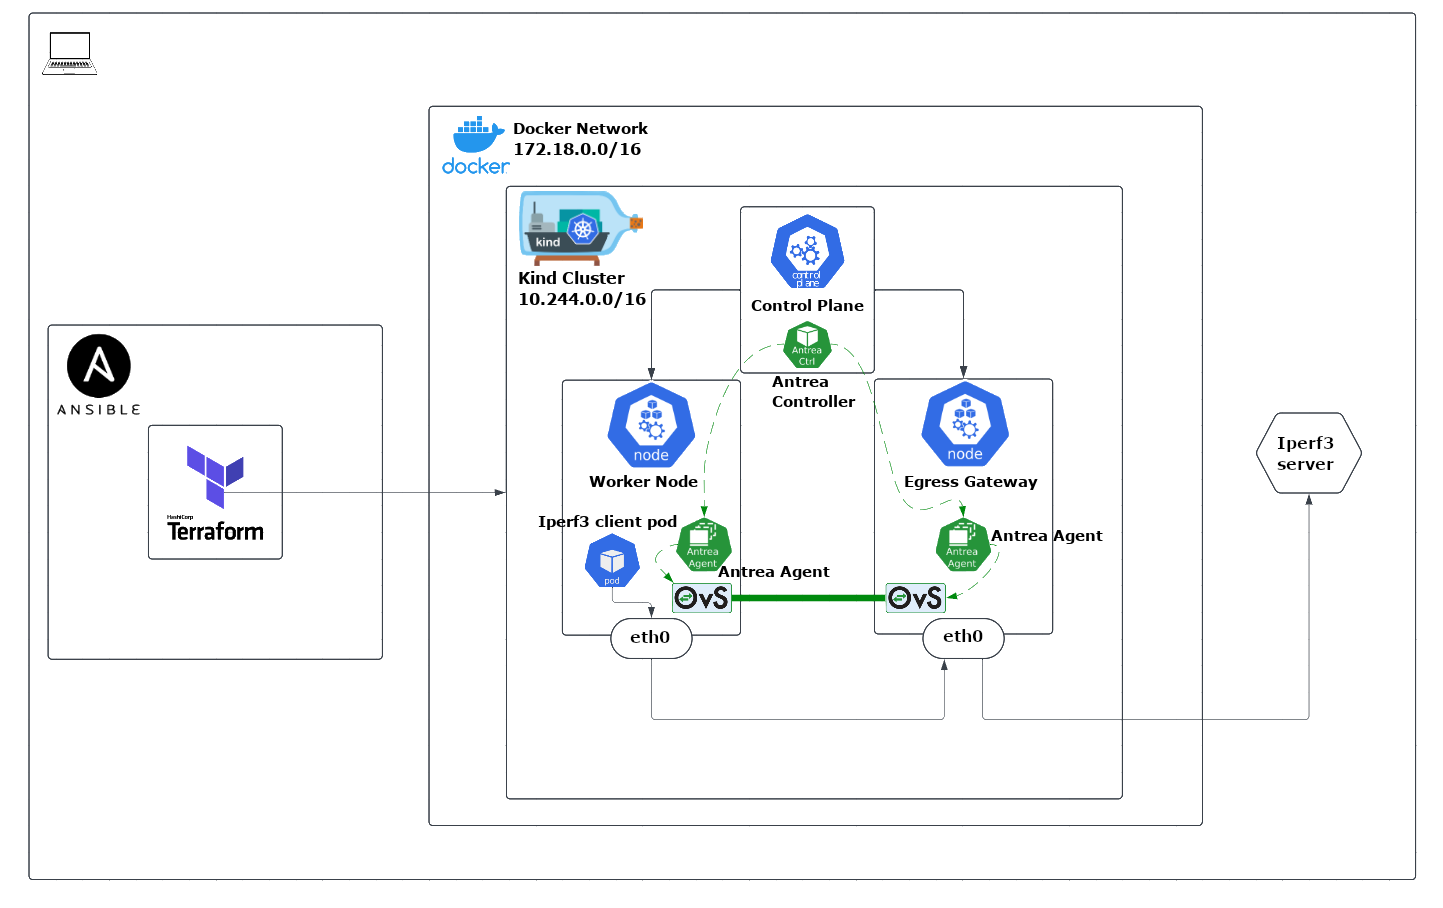
\includegraphics[width=1\columnwidth]{images/antrea_egress_gateway_cluster.png}
  \caption{Antrea Egress Scenario infrastructure \cite{AntreaDocs}\cite{NGINX}.}
  \label{fig:antreaEgressScenarioArch}
\end{figure}

The Kubernetes cluster, as shown in Figure~\ref{fig:antreaEgressScenarioArch}, is provisioned on a personal computer using Kind and configured with Ansible and Terraform. The cluster consists of three nodes: a control plane, a worker node, and an egress gateway, all of which are part of the Docker network. When the role \textit{terraform\_run\_egress\_iperf} starts execution and the created Iperf3 pod is ready, the test begins. The client, using the TCP protocol, sends data to the server (outside the cluster), which is routed through the egress gateway. The Iperf3 server detects that the traffic is coming from the egress gateway node (it sees the IP address of the egress gateway node as the source), because the traffic from the pod is SNATed. The Iperf3 client sends data packets using the TCP protocol, and after receiving acknowledgment from the server, the networking metrics are stored in memory. At the end of the test, a JSON file containing the gathered data is saved inside the pod. This file is saved on a volume shared with the host (personal laptop), ensuring that the data remains accessible after the test ends and the pod is terminated. Meanwhile, the Node Exporter continuously scrapes the metrics, which are pulled by Prometheus into its database. After the measurement is complete, the unformatted data is downloaded from Prometheus and saved as a CSV file. 

\begin{figure}[H]
  \centering
  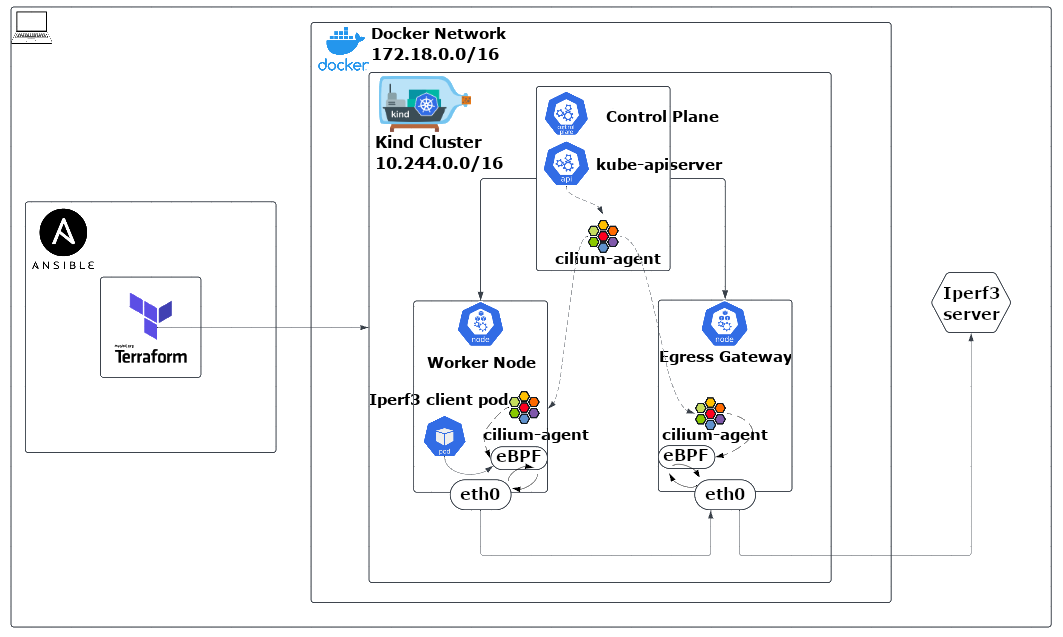
\includegraphics[width=1\columnwidth]{images/cilium_egress_gateway_cluster.png}
  \caption{Cilium Egress Scenario infrastructure \cite{CiliumDocs}.}
  \label{fig:ciliumEgressGatewayScenarioArch}
\end{figure}

The playbook for Cilium is similar to the one used to create the egress scenario with the Antrea CNI. The Ansible roles are designed to be reusable across different playbooks. The only differences are the CNI installation, the deployment of the Egress Gateway, and in Cilium, the desired node is labeled with \textit{egress-node=true} \cite{CiliumDocs}. The infrastructure can be seen in Figure~\ref{fig:ciliumEgressGatewayScenarioArch}. The Iperf3 pod starts generating traffic, which is encapsulated and sent to the egress gateway. The gateway performs IP address translation and forwards the data to the Iperf3 server outside the cluster.


%---------------------------------------------------------------------------

\section{Ingress scenario implementation}
\label{sec:ingressImpl}

The ingress scenario evaluates the CPU and memory usage of the Antrea and Cilium Container Networking Plugins while using the Gateway API to handle weighted traffic routing. The experiment involves using the Gateway API to route 40\% of incoming requests to one pod and evaluating the accuracy of traffic splitting by two different Gateway APIs. The test setup includes the K6 load testing tool running outside the Kubernetes cluster, generating traffic towards the Gateway API. The simulated traffic has four intensity levels, determined by allocating different numbers of virtual users interacting with the Gateway API. These levels are one, ten, one hundred, and one thousand virtual users. The traffic is initiated using the K6 tool, which runs inside a container on a personal computer. The network generator performs HTTP requests to the Gateway API and saves the received responses, extracting the pod name to a text file (one per line). By compiling a list of responses containing the names of two pods, the accuracy of the Gateway API traffic splitting is calculated. CPU and memory usage are monitored with a Node Exporter throughout the test and retrieved at the end of the scenario.


%---------------------------------------------------------------------------
\subsection{Cluster provisioning}
\label{sec:clusterProvisioning}

Creating a local cluster using Kind is a straightforward process, as described earlier. However, when setting up a Kubernetes cluster on Azure, the azurerm (\textit{Azure Resource Manager}) Terraform provider must be properly configured to authenticate with an Azure account. The script shown in Listing~\ref{lst:terraformScript} is responsible for creating the Kubernetes cluster in Azure Services. It is important to choose an appropriate location for the cluster, define the default node pool (including virtual machine type and node count), and remove the default CNI by setting the \textit{network\_plugin} in the \textit{network\_profile} to "none" if a different networking plugin is preferred \cite{AKS}.

\begin{listing}[htb]
  \centering
  \caption{Terraform Azure Kubernetes Service creation script \cite{AKS}.}
  \begin{minted}[gobble=4, frame=single, linenos, fontsize=\scriptsize]{hcl}
    resource "azurerm_resource_group" "rg" {
      location = var.resource_group_location
      name     = "rg${var.common_infix}"
    }

    resource "azurerm_kubernetes_cluster" "k8s" {
      location            = azurerm_resource_group.rg.location
      name                = "cluster${var.common_infix}"
      resource_group_name = azurerm_resource_group.rg.name
      dns_prefix          = "dns${var.common_infix}"

      identity {
        type = "SystemAssigned"
      }

      default_node_pool {
        name       = "agentpool"
        vm_size    = var.vm_type
        node_count = var.node_count
      }

      linux_profile {
        admin_username = var.username

        ssh_key {
          key_data = azapi_resource_action.ssh_public_key_gen.output.publicKey
        }
      }

      network_profile {
        network_plugin    = "none"
        load_balancer_sku = "standard"
      }
    }
  \end{minted}
  \label{lst:terraformScript}
\end{listing}


%---------------------------------------------------------------------------
\subsection{Infrastructure}
\label{sec:infra}

The process of creating an ingress scenario with Antrea CNI on Azure Kubernetes Services is fully automated showed in Listing~\ref{lst:antreaIngressPlaybook}. The script provisions the infrastructure seen in Figure~\ref{fig:antreaIngressScenarioArch}. The steps in the scripts are: 


\begin{enumerate}
  \item create\_azure\_cluster -- Runs Terraform to provision infrastructure in the cloud and configures the local environment to allow kubectl to interact with the cluster.
  \item install\_antrea -- Installs Antrea CNI plugin.
  \item wait\_until\_antrea\_installed -- Waits until Antrea is installed.
  \item install\_gateway\_api\_crd -- Applies custom definition resources, Gateway, GatewayClass, HTTPRoutes etc.
  \item install\_nginx\_gateway\_fabric -- Installs NGINX Gateway Fabric using Helm and waits until is ready.
  \item deploy\_antrea\_ingress\_scenario -- Deploys the ingress scenario (echo pods and Gateway API) using Terraform.
  \item monitoring -- Enables monitoring with Node Exporter and Prometheus.
  \item register\_gateway\_api\_ip -- Registers the IP address of the Gateway API for the K6 tool.
  \item run\_k6 -- Creates a container with K6, which generates HTTP traffic accessing Gateway API.
  \item scrap\_prometheus\_data -- Downloads data about CPU and memory utilization.
\end{enumerate}

\begin{listing}[H]
  \centering
  \caption{Ansible playbook used to deploy Antrea with Gateway API \cite{AnsibleDocs}.}
  \begin{minted}[gobble=4, frame=single, linenos, fontsize=\scriptsize]{yaml}
    - name: Create antrea ingres scenario with gateway api
      hosts: "{{ target | default('localhost') }}"
      vars_files:
        - ./vars/antrea.yml
        - ./vars/cloud.yml
        - ./vars/common.yml
        - ./vars/traffic_splitting.yml

      roles:
        - create_azure_cluster
        - install_antrea_cloud
        - wait_until_antrea_installed
        - install_gateway_crd
        - install_nginx_gateway
        - deploy_antrea_ingress_scenario
        - monitoring
        - register_gateway_api_ip
        - run_k6
        - scrap_prometheus_data
  \end{minted}
  \label{lst:antreaIngressPlaybook}
\end{listing}


\begin{figure}[tbh]
  \centering
  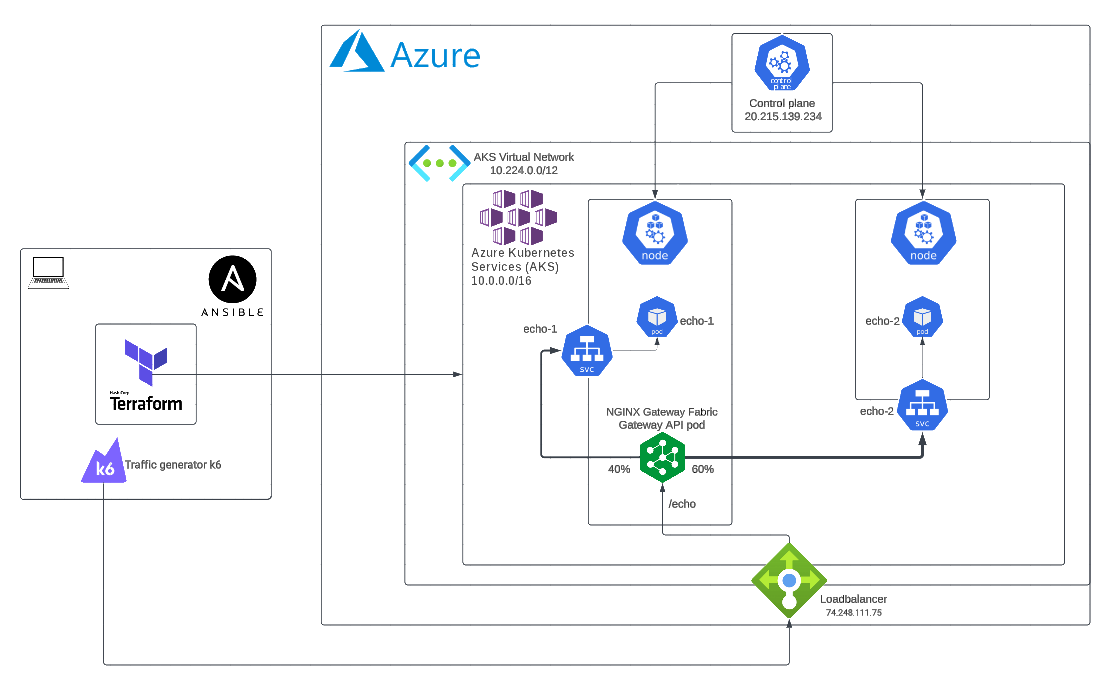
\includegraphics[width=1\columnwidth]{images/antrea_cloud_traffic_splitting.png}
  \caption{Antrea Ingress Scenario infrastructure \cite{NGINX}\cite{K6}.}
  \label{fig:antreaIngressScenarioArch}
\end{figure}

Figure~\ref{fig:antreaIngressScenarioArch} shows the cluster created using the script from Listing~\ref{lst:antreaIngressPlaybook}. In the cloud environment, the NGINX Gateway API pod is located on one of the nodes, which also runs the echo pod. Communication between the two pods within the node occurs via the Open vSwitch (OvS) bridge \cite{AntreaDocs}. In the local infrastructure, the gateway is forced to be deployed on the control plane node, so it uses Node-to-Node communication when routing traffic. Since Cilium uses the Gateway API, which does not run in a pod, the resource utilization is distributed between both nodes to Envoy.

%---------------------------------------------------------------------------


\begin{figure}[H]
  \centering
  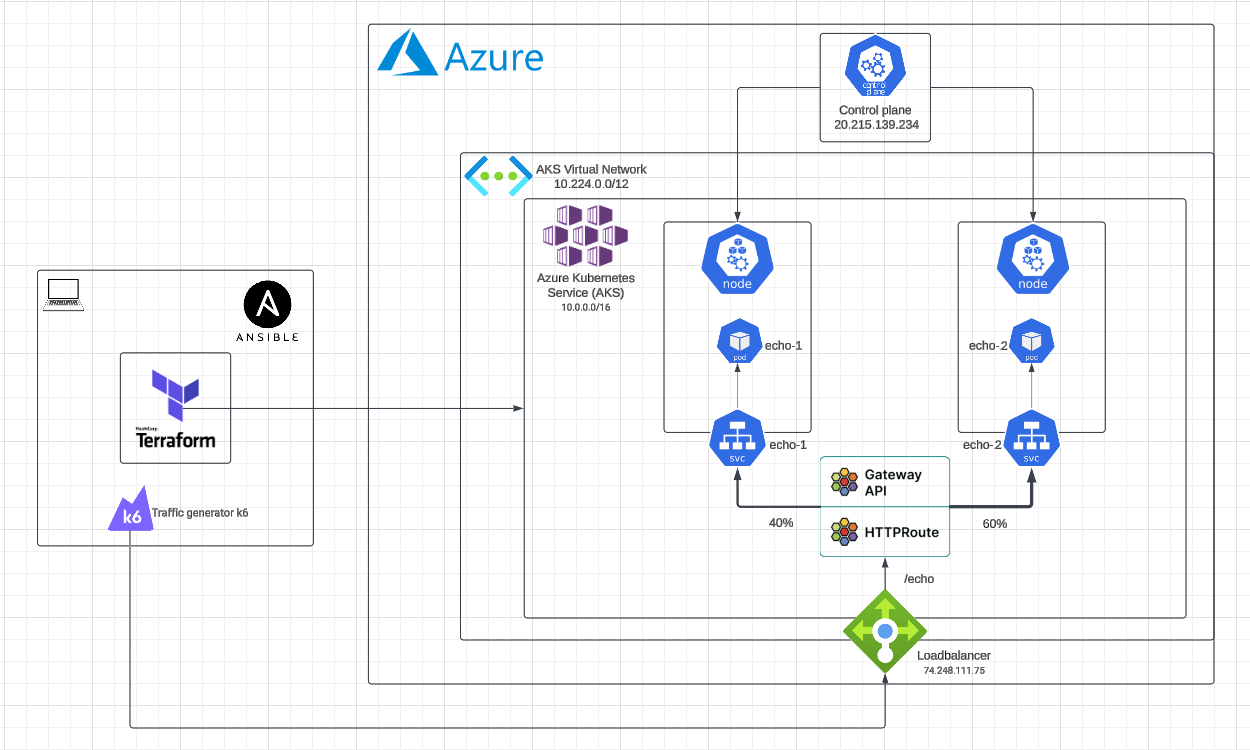
\includegraphics[width=1\columnwidth]{images/cilium_cloud_traffic_splitting.png}
  \caption{Cilium Ingress Scenario infrastructure \cite{CiliumDocs}\cite{CiliumUseCases}.}
  \label{fig:ciliumIngressScenarioArch}
\end{figure}

Both test cases, shown in Figures~\ref{fig:antreaIngressScenarioArch} and~\ref{fig:ciliumIngressScenarioArch}, consist of two nodes, each running echo pods. The pods host an application designed to return their pod name when a request is made to the "/echo" endpoint. The Grafana K6 tool sends requests to the exposed Gateway API IP address and, in return, logs which pod responded to the request. This information is used to calculate the accuracy of traffic weighting in both configurations. The load balancer shown at the bottom of the figures exposes the Gateway API to a public IP address so that the K6 client, located on a personal computer, can perform the requests. It does not split the traffic; that is done by the Gateway API.

The ingress scenario using the Cilium CNI plugin does not require the installation of NGINX Gateway Fabric, as it utilizes its own built-in implementation.

%---------------------------------------------------------------------------

\subsection{The differences between cloud and local runs}
\label{sec:diff}

\subsubsection{Control plane}
\label{sec:cplaneDiff}

In the local environment, the control plane node is created in the same way as the worker nodes, running as a container. However, when using NGINX with the Antrea CNI, the NGINX Gateway Fabric pod is deployed on a separate control plane node. This setup allows the routing of traffic between two different nodes, ensuring that traffic always exits the node. In contrast, when using AKS (Azure Kubernetes Service), the control plane is not part of the node pool; it is a separate managed service outside the node pool, providing a clearer separation between the control plane and worker nodes. This architectural difference can affect the measurements (compared to the local stack), as resource utilization of the control plane node is not gathered.

\subsubsection{Client traffic generator}
\label{sec:clientServerDiff}

In the cloud setup, the client running on a personal computer generates HTTP requests to the public Gateway API IP address exposed by Azure Cloud. Resource utilization within the cluster is exclusive to the cluster itself, not the client. However, when running the local stack, the client is part of the laptop on which the cluster is running, which could influence the measurements.
